\begin{frame}{Allgemeines}{Über Linked Lists}
	\begin{itemize}
		\item Simple Listenstruktur
		\item Elemente können verteilt im Speicher liegen
		\item Jedes Element speichert einen Datenwert
		\item ...und eine Referenz zum Nachfolger
		\item Speichern mehrdimensionaler Daten theoretisch möglich
		\begin{itemize}
			\item Wenn der Datenwert auch wieder eine Linked List ist
			\item Zugriff allerdings weniger intuitiv als im Array
		\end{itemize}
	\end{itemize}
\end{frame}


\begin{frame}{Eigenschaften}{Von Linked Lists}
	\begin{itemize}
		\item Muss keinen fortlaufenden Teil im Speicher belegen
		\item Dadurch entfallen einige Nachteile des Arrays:
		\begin{itemize}
			\item Größe muss nicht bei Initialisierung bekannt sein
			\item Liste kann dynamisch wachsen bzw. schrumpfen (Ohne "`teuere"' Kopiervorgänge)
			\item Einfügen bzw. Entfernen ist schneller
		\end{itemize}
		\item Allerdings ist der Zugriff auf Elemente langsamer
	\end{itemize}
\end{frame}

\begin{frame}{Datenstruktur von Linked Lists}{Listenelemente (Vgl. \cite{fahr:list})}
	\begin{itemize}
		\item Jedes Element einer Linked List ist ein Objekt
		\item Jedes Objekt vom Typ \textit{ListElement} besteht aus:
		\begin{itemize}
			\item Einem Member das den Wert des aktuellen Elements speichert. Datentyp ist der Typ, den die Liste speichert (\texttt{Double}, \texttt{Integer} etc.)
			\item Einem Member welches das nächste Element (bzw. eine Referenz darauf) in der Liste repräsentiert. Datentyp ist hier \texttt{ListElement}
		\end{itemize}
		\item Gibt es kein nächstes Element in der Liste kann dies über ein spezielles \texttt{tail} Objekt oder eine \texttt{null} Referenz dargestellt werden
	\end{itemize}
\end{frame}

\begin{frame}{Datenstruktur von Linked Lists}{Liste (Vgl. \cite{fahr:list})}
	\begin{itemize}
		\item Die Liste vom Typ \texttt{LinkedList} besteht an sich lediglich aus:
		\begin{itemize}
			\item Einem Member \texttt{head}(Auch: \texttt{first}, \texttt{top} o.Ä.) vom Typ \texttt{ListElement}, welches das erste Element der Liste repräsentiert.
			\item Den für die Liste benötigten Operationen zum Zugriff und Manipulation von Listenelementen
		\end{itemize}
		\item Sollte die Liste leer sein, so ist \texttt{head} ein Verweis auf \texttt{null} oder ein spezielles Element, das das Ende einer Liste repräsentiert.
	\end{itemize}
\end{frame}

\begin{frame}{Datenstruktur von Linked Lists}{Visualisiert}
%TODO: Visualisierung LinkedLists
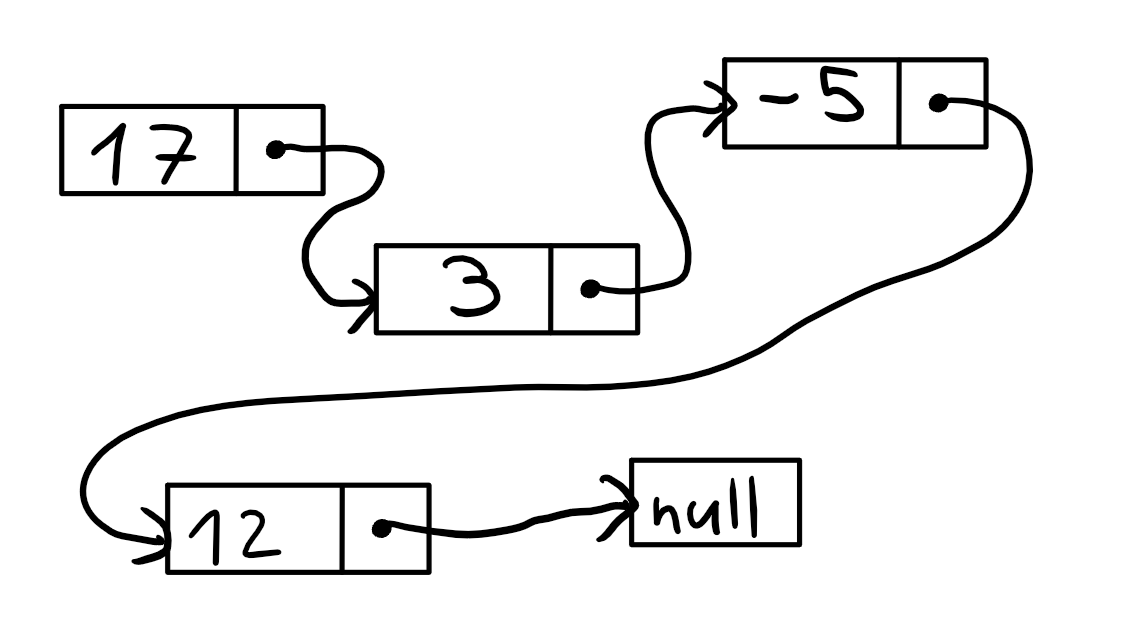
\includegraphics[height=6cm]{graph/llist_basic}
\end{frame}

\begin{frame}{Grundoperationen}{Anlegen einer Linked List}
	\begin{itemize}
		\item Bei Anlegen einer neuen Linked List wird diese als leere Liste initialisiert
		\item Anders als beim Array muss kein Speicher für die Listenelemente reserviert werden
		\item Das heißt, das \texttt{head} Element wird mit einer \texttt{null} Referenz initialisiert
		\item Das erste Element, das hinzugefügt wird, wird automatisch zum \texttt{head} Elemente der Liste
		\item Wird ein Element hinzugefügt, wird erst zum Zeitpunkt des Hinzufügens der Speicher für dieses Element reserviert
	\end{itemize}
\end{frame}

\begin{frame}{Grundoperationen}{Zugriff auf Elemente (Vgl. \cite{fahr:list})}
	\begin{itemize}
		\item Zugriff auf Elemente muss immer sequentiell vom \texttt{head} Element aus erfolgen
		\item Zugriff auf das $n$-te Element erfolgt durch wiederholtes Zugreifen auf das \texttt{next} Element
		\item Bedeutet:
		\begin{itemize}
			\item Je weiter hinten das gesuchte Element steht, desto mehr Operationen sind möglich
			\item Somit ergibt sich die Komplexität zu $O(N)$
		\end{itemize}
	\end{itemize}
\end{frame}

\begin{frame}[fragile]{Zugriff auf Listenelemente}{Mögliche Codeimplementierung}
\lstset{style=java}
\begin{lstlisting}
public T getElement(int index){
    ListElement res = head;
    for(int i=0;i<index;i++){
        res = res.getNext();
    }
    return res.getValue();
}
\end{lstlisting}
\end{frame}

\begin{frame}{Grundoperationen}{An-/Einfügen von Elementen}
	\begin{itemize}
		\item Nachträgliches Einfügen vergleichsweise simpel
		\item Dadurch, dass Elemente an beliebigen Stellen im Speicher liegen
		\item Dadurch kein neuanlegen der Liste notwendig
		\item Oder kopieren von Elementen
		\item Beim Einfügen werden lediglich die Referenzen der Listenelemente aktualisiert
	\end{itemize}
\end{frame}

\begin{frame}{Grundoperationen}{Komplexität beim Einfügen}
	\begin{itemize}
		\item Komplexität auch hier $O(i)$
		\begin{itemize}
			\item $i$ bezeichnet hier die Position an der Liste in der eingefügt wird
			\item Somit ist das Einfügen hier (anders als bei Array) von der Länge der Liste unabhängig
		\end{itemize}
		\item Selbst ein Einfügen an letzter Position ist aber in der Regel schneller als in Arrays
		\begin{itemize}
			\item Da keine Kopieroperationen durchgeführt werden müssen
		\end{itemize}
	\end{itemize}
\end{frame}

\begin{frame}{Einfügen von Elementen}{Visualisiert}
%TODO: Abbildung einfügen von Elementen
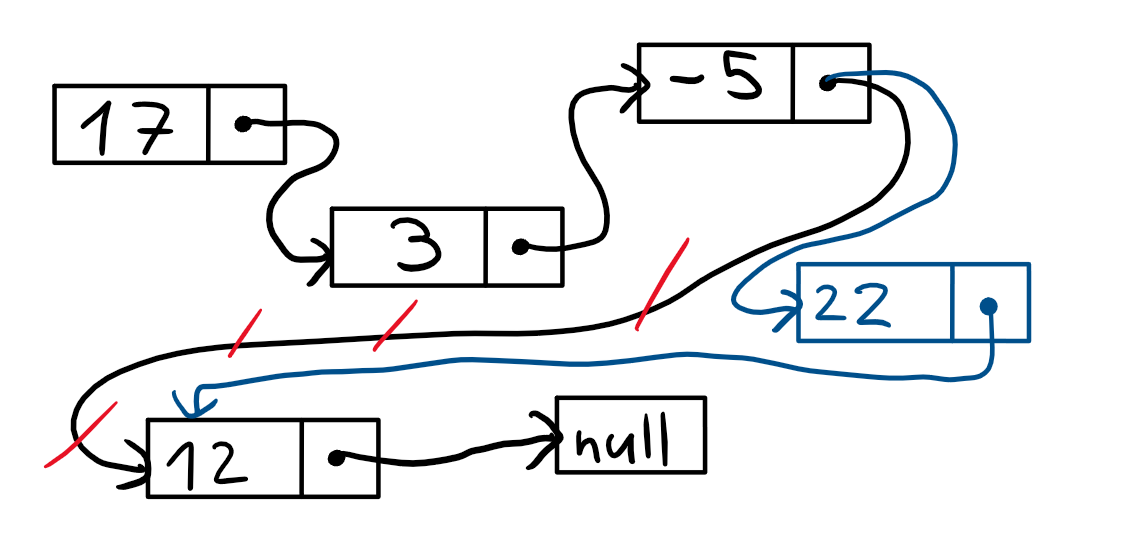
\includegraphics[height=6cm]{graph/llist_insert}
\end{frame}

\begin{frame}{Grundoperationen}{Zählen von Elementen}
	\begin{itemize}
		\item Anders als beim Array kann Länge alleine aus Listenelementen ermittelt werden
		\item Dadurch, dass das Ende der Liste über eine \texttt{null} Referenz erkennbar ist
		\item Vorgehen im Groben(Siehe Struktogramm auf nächster Folie):
		\begin{itemize}
			\item Ausgehend vom \texttt{head} Element, erhöhe den Zähler solange, wie es ein \texttt{next} Element gibt
		\end{itemize}
		\item Komplexität ist somit $O(N)$
		\item In der Regel wird die Länge jedoch als \texttt{int} von der Liste gespeichert und bei Hinzufügen/Entfernen aktualisiert
	\end{itemize}
\end{frame}

\begin{frame}{Zählen von Elementen}{Struktogramm}
\begin{centernss}
	\begin{struktogramm}(70,30)
        \assign{Setze \( curElement=head \) }
        \assign{Setze \( count=0 \) }
        \while{\( curElement!=null\) }
			\assign{curElement=curElement.next}
			\assign{count++}
		\whileend
		\assign{Gib \( count \) zurück}
	\end{struktogramm}
\end{centernss}
\end{frame}

\begin{frame}{Grundoperationen}{Entfernen von Elementen}
	\begin{itemize}
		\item Elemente müssen nicht sequentiell im Speicher liegen
		\begin{itemize}
			\item Dadurch entsteht keine "`Lücke"' in der Liste
		\end{itemize}
		\item Dadurch ähnlicher Vorteil gegenüber dem Array wie beim Einfügen:
		\begin{itemize}
			\item Keine Kopieroperationen(der nachfolgenden Elemente) notwendig
		\end{itemize}
		\item Um ein Element zu entfernen muss lediglich das \texttt{next} Element des Vorgängers auf das \texttt{next} Element des
		zu entfernenden Elements geändert werden
		\item Entferntes Element liegt dann unreferenziert im Speicher $\rightarrow$ Wird in Java durch die Garbage Collection entfernt
		\item Komplexität ist hier wie beim einfügen von Elementen $O(i)$
	\end{itemize}
\end{frame}

\begin{frame}{Entfernen von Elementen}{Visualisiert}
%TODO: Visualisierung entfernen von Elementen
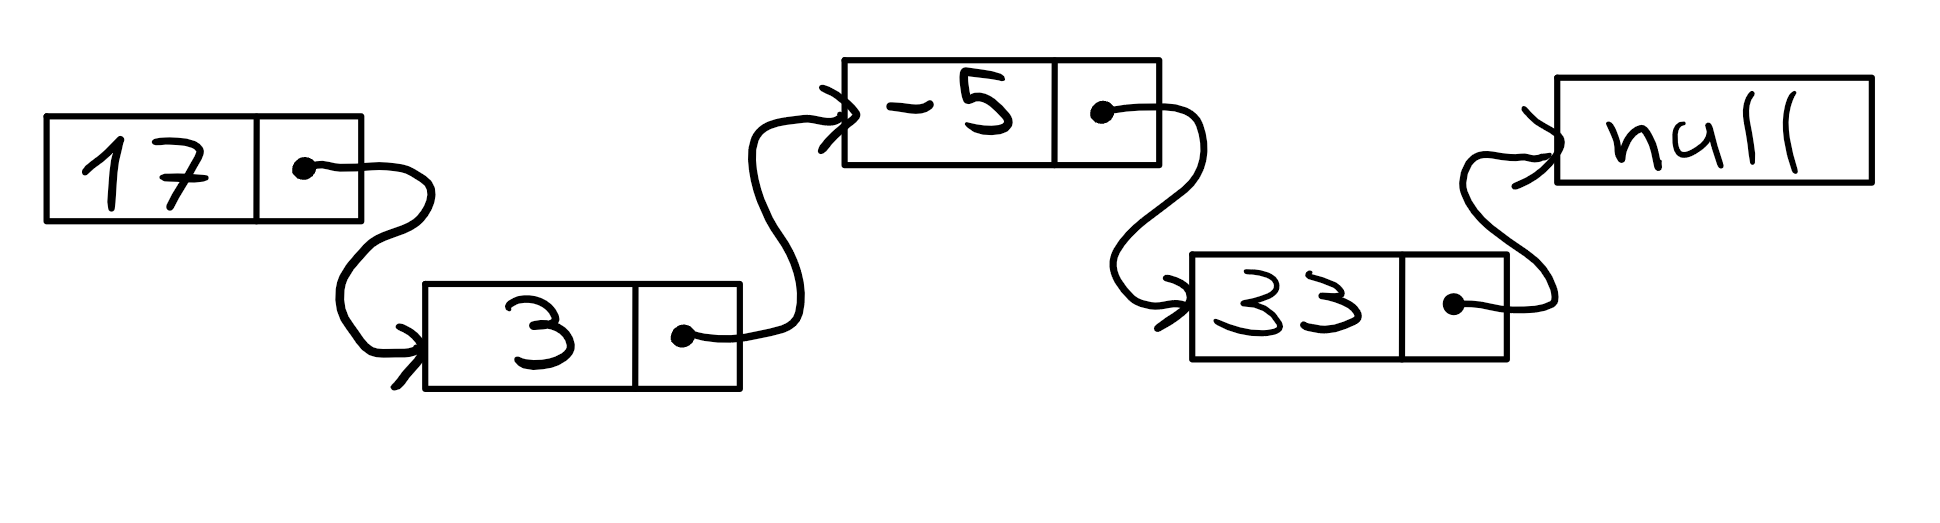
\includegraphics[width=.8\textwidth]{graph/llist_remove_pre}

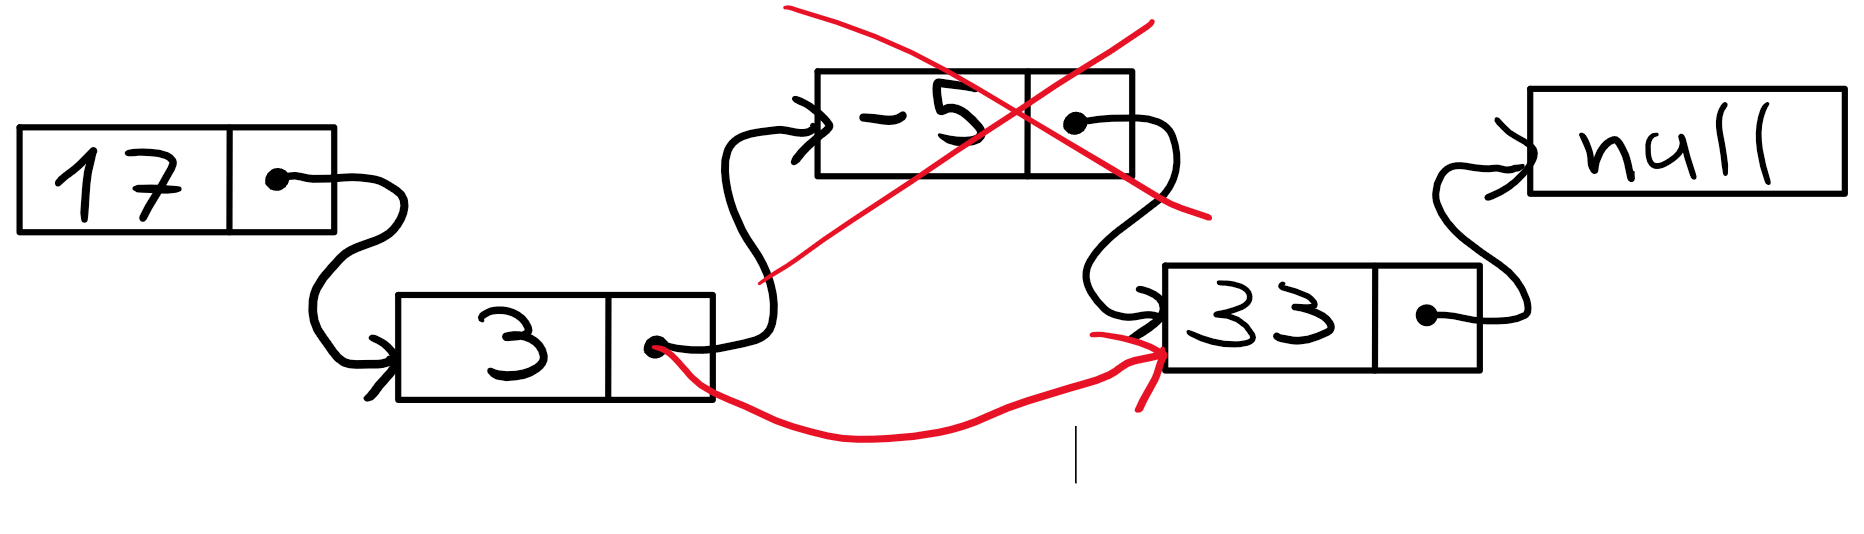
\includegraphics[width=.8\textwidth]{graph/llist_remove_post}
\end{frame}

\begin{frame}{Grundoperationen}{Konkatinieren von Listen}
	\begin{itemize}
		\item Kombinieren von Listen ist simpel
		\begin{itemize}
			\item Kein neuer/zusätzlicher Speicher muss reserviert werden
			\item Kopieren von Elementen nicht zwingend notwendig (Je nach Implementierung jedoch sinnvoll)
		\end{itemize}
		\item Zum konkatinieren muss lediglich die \texttt{next} Referenz des letzten Elements der ersten Liste aktualisiert werden
		\begin{itemize}
			\item Auf das \texttt{head} Element der zweiten Liste
		\end{itemize}
		\item Komplexität ist somit (theoretisch) $O(n)$ um bis zum letzten Element der ersten Liste zu gelangen
	\end{itemize}
\end{frame}

\begin{frame}{Konkatinieren von Listen}{Visualisiert}
%TODO: Visualisierung Konkatinieren von Listen
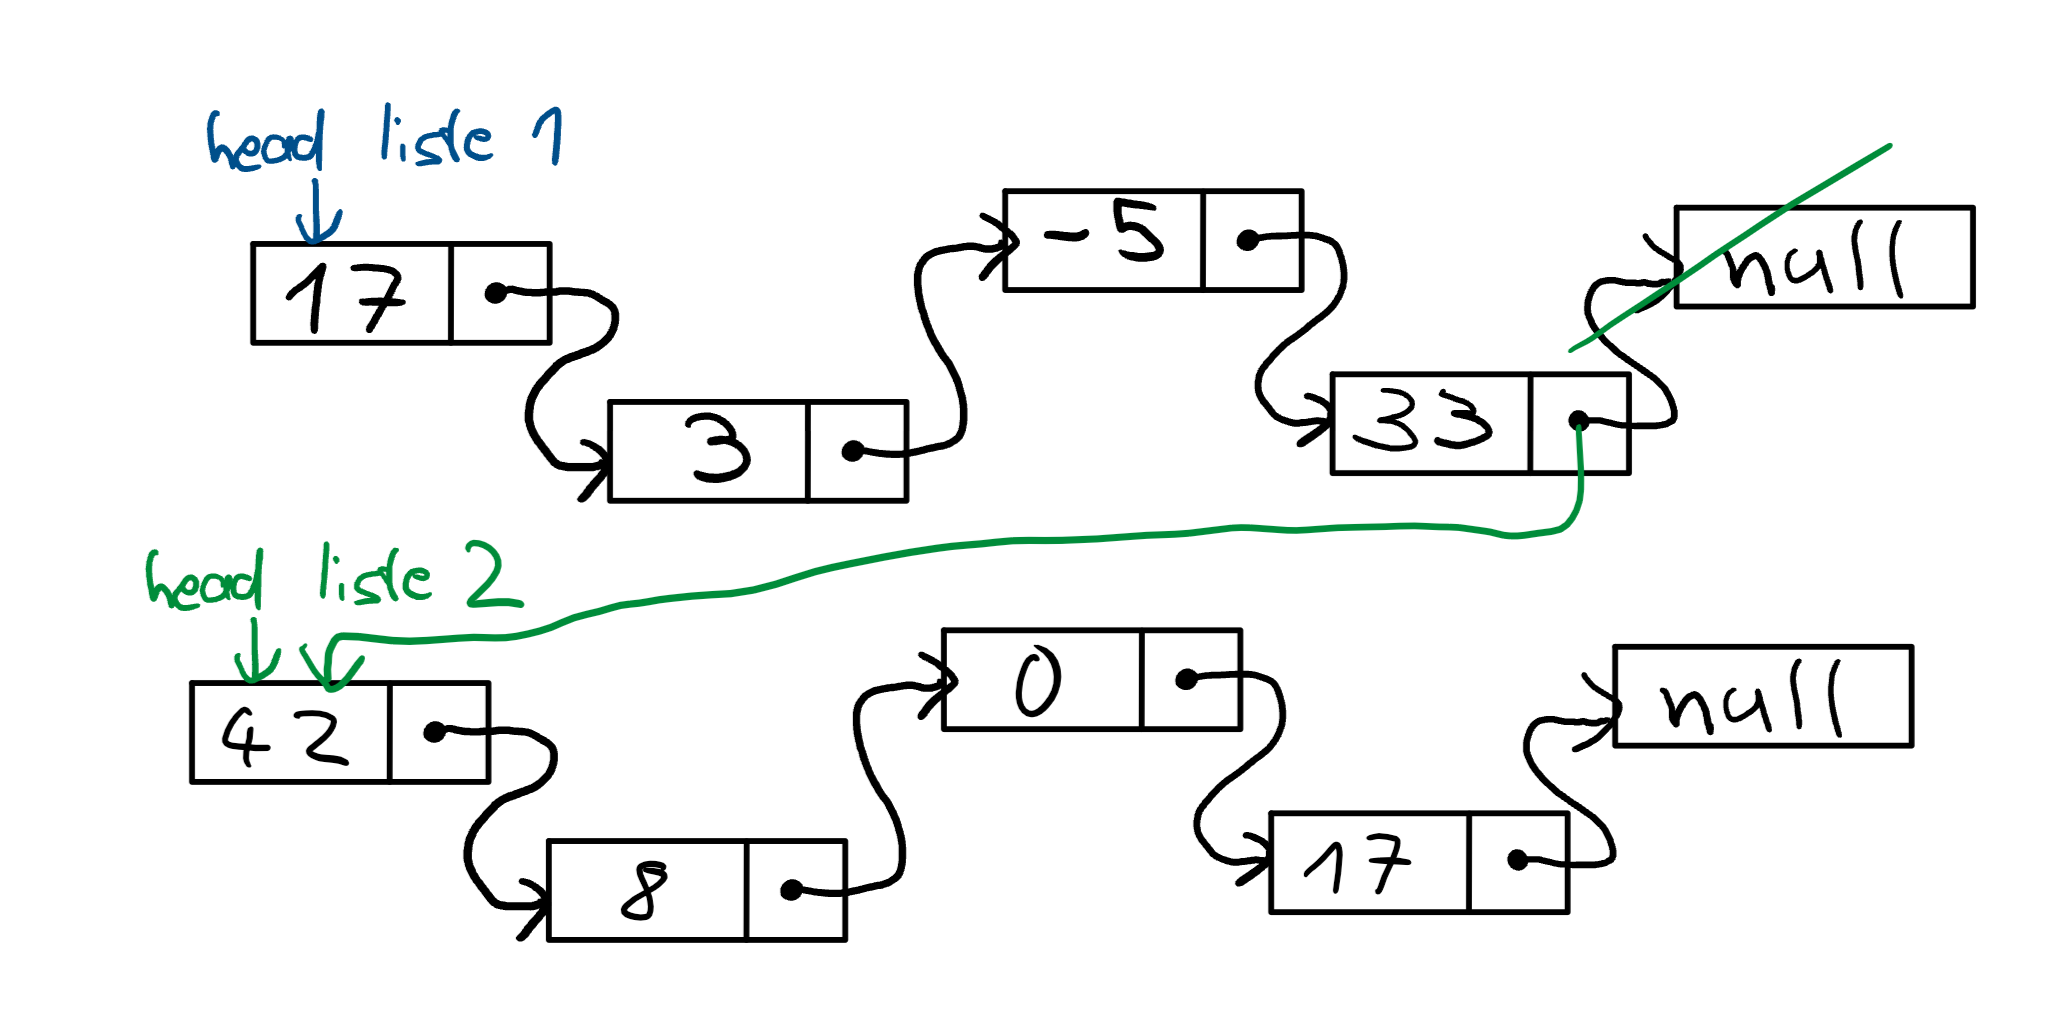
\includegraphics[width=.8\textwidth]{graph/llist_concatenate}
\end{frame}

